\documentclass[conference]{IEEEtran}
\usepackage{amsmath,amssymb,graphicx,url,flushend}
\def\UrlBreaks{\do\/\do-\do\_}
\graphicspath{{figures/}}
\providecommand{\MacroSstate}{0.9198}
\providecommand{\MacroSstateHist}{0.7144}
\providecommand{\MacroSpatialSstate}{0.8798}
\providecommand{\MacroSlink}{0.999931}
\providecommand{\MacroRefinedPanels}{10}

\newcommand{\EventSubmission}{58021199}
\newcommand{\EventPublicScore}{0.83220}
\title{CREST: Constrained Reconstruction and Estimation of Spatiotemporal Traffic}
\author{\IEEEauthorblockN{Arjun Vijay Prakash}\IEEEauthorblockA{Independent Researcher}}
\begin{document}
\maketitle
\begin{abstract}
TrafficFlowBench evaluates missing-state reconstruction, short-horizon queues,
physical consistency and path-flow estimation. We first built a reproducible
independent system of graph--temporal gradient boosting, wave-aware residuals,
conditioned queue localizers and a nonnegative demand solver, scoring 0.83220
on the public leaderboard. A subsequent public-source campaign compares
reconstruction algorithms on matched temporal blocks and evaluates attributed,
licensed checkpoint inference. A 50/50 blend of our state estimator and the
public anubisyy CatBoost ensemble, combined with its causal queue checkpoints
and our own OD solver, scores 0.86438. Adding an independently inferred MIT-licensed U-Net raises the composite to 0.87387. Controlled submissions isolate gains of
0.02557 from queue replacement and 0.00662 from state blending. We distinguish
these public comparisons from private generalization, which remains unknown,
and disclose the source, license and contribution of external models. Every
output is regenerated from the released observations and model checkpoints.
\end{abstract}
\begin{IEEEkeywords}
traffic state estimation, gradient boosting, queue forecasting, path flows, physical constraints
\end{IEEEkeywords}

\section{Introduction}
Freeway traffic state estimation must reconcile sparse sensing, multi-step
forecasting, physical feasibility, and origin--destination consistency under
a fixed upload contract. We document a complete participant pipeline for
TrafficFlowBench that compares neural and tree learners, selects models on
purged temporal validation, and emits a strict multi-task submission without
silent imputation.

\section{TrafficFlowBench benchmark}
TrafficFlowBench releases synthetic freeway observations generated by a
calibrated traffic model, rather than redistributing real detector records
\cite{bench}. Ten directional panels share four tasks. Task 1 predicts speed
$v$ and total link flow $q$ at template-enumerated missing cells. Task 2 predicts
binary queue membership at six five-minute horizons. Task 3 evaluates the same
Task 1 submission for physical consistency. Task 4 predicts nonnegative path
flows from released link counts and a weak path prior.

\textbf{Evaluation scope.} Training uses the official synthetic participant release through 28 February 2031. The initial retained subset has 6,948 files and 7.28 GB; redundant masked training files and unused templates are omitted. Both scored months are predicted. The omitted training masks/templates were restored from the official archive for the public-source comparison campaign. The initial submission \EventSubmission{} completed scoring on 5 November 2026 at \EventPublicScore{} public composite. Private and official task-level scores remain unavailable.

The released scoring weights are $0.35$, $0.30$, $0.15$, and $0.20$ for the
four tasks, respectively. These weights do not make an overall score locally
identifiable. Queue labels are withheld for every split; conservation requires
organizer-held boundary flows; and three of the four ODME components require
hidden path flows. Reporting their public proxies as official scores would
misrepresent what the release permits.

\section{Model design}
\subsection{Graph and temporal features}
Links form a directed graph read from the released mainline topology. An edge
from $i$ to $j$ has weight
\begin{equation}
 W_{ij}=A_{ij}\exp(-\tau_i/5),\quad
 \tau_i=60L_i/v_{f,i},
\end{equation}
where $L_i$ is in kilometers and $\tau_i$ in minutes. Separate normalized
upstream and downstream operators aggregate only finite observations. Missing
neighbors are excluded from the denominator. The system also constructs a
symmetric normalized graph Laplacian for inspection.

The tree features include twelve lagged states, upstream and downstream lag
aggregates, local observation masks, weekday and time-of-day encodings, and
released link attributes. Downstream--upstream speed differences describe local
congestion contrasts. A bounded estimate of $\Delta q/\Delta k$ describes a
kinematic-wave ratio, with small density differences excluded to prevent unstable
division. These are predictive features, not estimates of an observed shock speed.

\subsection{State reconstruction}
Graph-masked multihead attention allows each link to attend to itself and its
immediate upstream and downstream links. A one-layer temporal Transformer then
processes the resulting link histories. Graph attention follows the neighborhood
restriction used in graph attention networks \cite{gat}; the temporal architecture
here is a participant implementation rather than a reproduction of that model.
Directed graph traffic forecasting provides related motivation \cite{dcrnn}.

Artificial corruption removes both speed and flow at each selected link-time
cell. The neural reconstruction head predicts the center of a 25-step window,
so it can use released observations on either side of a Task 1 target. Separate
LightGBM regressors \cite{lgbm} learn the two normalized channels from the
corrupted training inputs. The ablation blend assigns tree and neural weights $0.8$ and $0.2$. The tree imputer fills missing cells and repeats its pass once. The earlier 0.76439 upload uses the residual refinement below on every corridor; the v4 revision adds the context features described later. The blend and the tree-only alternative are compared on the temporal holdout. The initial 80-round tree models use at most 60,000 sampled training cells per target. Neural comparison runs use one epoch of 60 minibatches, with the batch size reduced to two to fit system memory. Neural-only comparisons cover nine panels and are unavailable for D7\_I405\_S; the tables state coverage explicitly. The deployed policies do not use the neural component.

\subsection{Residual reconstruction refinement}
A second reconstruction model starts from two-sided linear interpolation of the released masked observations. For each channel, it predicts the residual between the training target and this interpolated value. Interpolation is computed independently within each fit or validation segment; masked target values are never restored to the inputs. The feature vector appends the interpolated speed and flow to the graph and temporal features. The residual regressors use 220 boosting rounds and at most 120,000 sampled cells, mixing masking rates of 20, 30, and 50 percent. A candidate replaces the original reconstruction only when its mean held-out score improves by more than 0.001. Accepted models are then refitted on all released training months. A higher-capacity pilot with 600 rounds and 300,000 sampled cells failed the required improvement on both comparison blocks and was rejected. The full refit omits an unused neural model when validation selects trees.

\subsection{Condition-aware queue forecasting}
The causal input grid is $[T-60,T]$, with targets $T+5$ through $T+30$.
Only released window history and, where selected, eligible observations exactly
at $T$ are permitted. Monthly reconstruction and later observations cannot feed
this branch. Task 2 excludes D12\_I405\_N/S.

The initial queue system used six horizon-specific classifiers or speed
regressors. Its onset proxy selector greedily retained the earliest qualifying
origin, concentrating first queue arrival at the final forecast step. We instead
enumerate admissible origins, randomize selection, and enforce 360-minute
within-condition spacing. A second sampler balances first-arrival steps as a
robustness check. Labels threshold observed training speed at $0.6v_f$;
they are not the withheld latent queue labels. Conditions use the twelve
visible steps ending at $T-5$, and each selected horizon contains a queue.

Separate LightGBM heads for onset and ongoing conditions share all six horizons
through a horizon-index feature. Inputs include graph--temporal speed/flow,
capacity-normalized demand, recent means and observation ages, two-hop spatial
evidence, occupancy, quality, and occupancy-derived density. A linear
occupancy conversion is calibrated on fitting rows and supplies density when
window history omits that column. Training mirrors a missing $T$ row or the
selected partially observed origin policy. Production preserves released quality
flags when measurement masking removes the origin values.

Each head uses 180 boosting rounds, 15 leaves, learning rate 0.04, and at most
300 sampled positives and 300 negatives per event. Inverse sampling weights
restore the per-window class distribution and equalize window contributions.
Up to 128 events per condition are sampled for final training. Decoder selection
compares calibrated thresholds with a ranked-region IoU surrogate,
\begin{equation}
 U(k)=\frac{\sum_{i\in A_k}p_i}{k+\sum_i p_i-\sum_{i\in A_k}p_i},
\end{equation}
where $A_k$ contains the top $k$ probabilities. This ratio of expectations
approximates, and is not identical to, expected IoU. Predictions are nonempty
because both published conditions require a queue in the horizon.

Policies and decoders were selected on October training proxies after fitting
June--September. November compared all eight queue corridors against refitted
existing classifiers and speed regressors. Candidate policies were then frozen,
refitted before January, and assessed on January proxies. Feature-boundary
corrections were completed before the January experiment. A candidate must
improve condition-macro IoU by at least 0.05 under both samplers, retain ongoing
IoU within 0.02, and have a positive paired day-bootstrap 95\% lower bound.
Five corridors pass both stages. D7\_I10\_E is rejected despite a macro gain
because its January ongoing regression exceeds the limit. D7\_I10\_W and
D7\_I210\_E retain existing models after small November gains. Retained models
use history only; four accepted event models use origin observations and
D7\_I405\_S remains history-only. All selected models are finally refitted on
all released training months. If a retained classifier produces an empty window,
its highest-probability cell is selected. Both official conditions guarantee
nonempty truth, so this changes a zero-IoU prediction to one whose IoU is
nonnegative; it does not guarantee a positive intersection.

\begin{table}[t]\centering
\caption{Observed-speed queue proxy changes against refitted baselines. Entries are changes in condition-macro IoU on the random sampler. Both samplers and ongoing-regression gates determine retention.}
\label{tab:eventqueues}
\begin{tabular}{lrrl}\hline
Panel & Nov. $\Delta$ & Jan. $\Delta$ & Policy \\ \hline
D12\_I5\_N & +0.177 & +0.214 & event \\
D12\_I5\_S & +0.099 & +0.088 & event \\
D7\_I10\_E & +0.196 & +0.189 & retained \\
D7\_I10\_W & +0.023 & -- & retained \\
D7\_I210\_E & +0.023 & -- & retained \\
D7\_I210\_W & +0.081 & +0.077 & event \\
D7\_I405\_N & +0.297 & +0.305 & event \\
D7\_I405\_S & +0.098 & +0.078 & event \\
\hline\end{tabular}\end{table}

These retrospective assessments participate in model retention and are
selection evidence, not an untouched test of the final selected system. The two
samplers share a month and do not constitute independent temporal folds.

\section{Physical constraints and inverse estimation}
\subsection{Fundamental-diagram feasibility}
The system reads calibrated fundamental-diagram parameters using the official
evaluator's parameter aggregation. Let $C$ be total link capacity, $k_j$ jam
density, and $k_c=C/v_f$. The triangular backward-wave parameter is
$w=C/(k_j-k_c)$. For a fixed feasible speed, the congested-branch inequality
has a closed form:
\begin{equation}
 q\leq w(k_j-q/v)
 \quad\Longleftrightarrow\quad
 q\leq\frac{wk_jv}{v+w}.
\end{equation}
The projection clips $v$ to $[1,v_f]$ and $q$ to
$[0,\min(C,wk_jv/(v+w))]$. It is a fixed-speed feasibility map,
not a Euclidean joint projection or a Greenshields fit. A piecewise
differentiable version contributes a small neural training penalty.

Density is then defined as $k=q/v$. This makes $q=kv$ an identity and does not
establish vehicle conservation. For example, doubling flow while holding speed
constant doubles inferred density even if the net boundary flux is zero.
Conservation instead requires
\begin{equation}
 L[k(t+1)-k(t)]=\Delta t
 [q_{\mathrm{in}}(t)+r_{\mathrm{on}}(t)-q_{\mathrm{out}}(t)-r_{\mathrm{off}}(t)].
\end{equation}
An optional sparse least-squares adjustment changes missing cells while keeping
observed cells fixed and penalizes this residual against topology-derived fluxes.
It excludes boundaries, latent unobserved neighbors, and unavailable attached
ramps. A structural absence of a ramp permits zero ramp flow; a missing ramp
measurement does not. This adjustment is disabled by default because the
organizer documentation states that topology-derived fluxes do not resolve the
official conservation signal. Near-zero official conservation error cannot be
guaranteed from released inputs.

\subsection{Nonnegative path-flow estimation}
The incidence matrix $A$ uses the released path and link identifiers. Duplicate
incidence pairs are removed. The solver estimates path flows by
\begin{equation}
 \hat f=\arg\min_{f\geq0}
 \|A_{\mathcal O}f-c_{\mathcal O}\|_2^2+
 \lambda\|f-b\|_2^2,
\end{equation}
where $\mathcal O$ contains only links with finite released counts and $b$ is
the weak prior for that split and departure-period token. The regularization is initially fixed at $\lambda=0.05$. Direct path-space solvers encountered iteration limits on the larger, correlated path sets. The implementation instead minimizes the equivalent link-space dual
\begin{equation}\begin{split}
h(u)={}&\tfrac12\|u\|_2^2+c_{\mathcal O}^{\mathsf T}u\\
&+\tfrac{\lambda}{2}\|[b-A_{\mathcal O}^{\mathsf T}u/\lambda]_+\|_2^2.
\end{split}\end{equation}
The primal solution is $f=[b-A_{\mathcal O}^{\mathsf T}u/\lambda]_+$. A semismooth Newton step uses the positive-definite generalized Hessian $I+A_{\mathcal O,\mathcal P}A_{\mathcal O,\mathcal P}^{\mathsf T}/\lambda$, where $\mathcal P$ is the positive path set. Cholesky solves and backtracking avoid constructing a dense path-by-path Hessian. Small-problem tests compare this dual result against primal nonnegative least squares. Unobserved connectors contribute no artificial zero-count constraints. The result need not fit counts exactly because nonnegativity and the weak prior also constrain it.

\section{Validation and reproducibility}
An 80/20 chronological cutoff separates fitting from validation. Both sides
exclude an 18-step interval around the cutoff, covering the 12-step history
and six-step forecast target. Feature construction operates separately within
each temporal segment. Preprocessing and model fitting cannot inspect the
held-out segment. Validation masks all measured channels together at rates
$0.2$, $0.3$, and $0.5$, corresponding to the three released mask regimes.
To bound CPU inference cost, the temporal experiment evaluates the last seven days of the held-out block. Artificial masks provide controlled reconstruction tests but do not reproduce
every property of the official template selection.

The separate spatial experiment leaves out an entire corridor family,
including both directions, and fits a shared tree model on the other families'
early training blocks. Its test set is the held-out family's later block.
This experiment evaluates transfer of the tree features. It must not be
reported as spatial validation of the separately fitted tree and residual reconstruction models.

For Task 1, validation reports speed RMSE, per-lane flow RMSE, and
\begin{equation}
 \begin{split}
 S_{state}={}&0.54\max(0,1-\mathrm{RMSE}_v/25)\\
 &+0.46\max(0,1-\mathrm{RMSE}_{q/lanes}/600).
 \end{split}
\end{equation}
Regimes are averaged within each panel, then directions within each family,
then families equally. The figures and table are generated from saved arrays
and metric files, rather than manually transcribed numbers.

The checkpoint manifest records the original BLAS inference thread count for each state model. Changing reduction order can move a few factor features across tree thresholds; reproduction pins these settings before comparing predictions. This is an inference reproducibility constraint, not additional fitting.

The strict upload builder preserves the six template columns and submission-ID
order. It checks nonnegative finite values, binary queue indicators, natural-key
uniqueness, and complete coverage. A missing prediction raises an exception
instead of silently emitting a zero. Both validation and private months must be
present before the final upload is produced. Fixture uploads receive a distinct
filename and remain inside the fixture artifacts folder.


\section{Fourth revision: conditional onset and cross-sensor state context}
\subsection{Onset timing and spatial localization}
The organizer confirms in the public discussion\footnote{\url{https://www.kaggle.com/competitions/2026-ieee-big-data-traffic-flow-bench/discussion/742350}} that onset windows have no queue at the first five forecast steps and a nonempty queue at the sixth, and permits conditioning on this contract. We enforce this support exactly. The localizer combines gradient-boosted probabilities, nearest training-event retrieval, and a training-only link prior. It adds normalized link-identifier index, directed degree, and causal occupancy/quality context to the earlier queue features. October selects the observation-at-origin policy, tree/retrieval/prior mixture, and decoder. November and January compare the chosen localizer with a timing-corrected classifier using the same fitting prefix. Five panels promote the localizer; three retain the corrected classifier. Production refits use the nine training months. Ongoing forecasts remain unchanged from submission 57833935. The timing and locality update changes 574 binary cells and raises the public composite from 0.76439 to 0.82716 in submission 57846489. Because all other fields are identical, the 0.06277 gain is attributable to queue predictions; it does not reveal an absolute queue score.

\subsection{Cross-sensor residual reconstruction}
A rank-ten factor model learns standardized cross-link speed/flow covariance from training observations. At inference, ridge regression estimates factors using only finite inputs in each masked row. Factors supply context to residual trees; they do not replace observations or introduce hidden targets. Additional features include distances to previous and following visible observations, interpolated upstream/downstream states, local Gaussian temporal summaries, and normalized link-identifier index. The residual learners use 300 boosting rounds and at most 160,000 training targets. Daily corruption draws one of the released 20, 30, or 50 percent missingness rates. The fit prefix ends before October; October 15--21 selects residual and factor blending weights. November and January 15--21 apply retention gates with those weights frozen. Every panel selects the enhanced residual alone, without a direct factor blend, and improves on both later blocks. The factor remains an input feature.

\begin{table}[t]\centering
\caption{State development scores, equally averaged over regimes, directions within family, and families. These previously examined months are retention evidence, not independent tests.}
\begin{tabular}{lcc}\hline
Block & Earlier residual & Enhanced residual\\\hline
November & 0.91575 & 0.93446 \\
January & 0.91094 & 0.93084 \\
\hline\end{tabular}\end{table}

\subsection{OD identifiability audit}
The observed path-incidence systems have only 35--100 independent constraints for 630--5050 candidate paths, so a close link-count fit cannot identify path truth. An entropy projection worsens held-out-link relative error, 0.0291 versus 0.0214, but improves error under a synthetic lognormal prior corruption, 0.2464 versus 0.3376. It fails the predeclared dual improvement gate, and additive regularized estimation remains deployed. Synthetic prior experiments do not establish behavior against hidden official paths.

\section{Earlier ablations and current official result}
The earlier residual reconstruction policy achieved family-macro $S_{state}=\MacroSstate{}$ on the purged artificial-mask holdout, against \MacroSstateHist{} for the historical-mean reference. The generated tables report the saved ablations and selected per-panel predictions. Model selection uses these same validation measurements, so the selected result has selection optimism. The final private month remains unlabeled and was used only for prediction.

\begin{table}[t]
\caption{Family-macro artificial-mask holdout scores. Panel coverage varies, so partial-panel scores are not directly comparable with ten-panel scores. Model selection uses this same validation set.}
\centering\begin{tabular}{llrr}
\hline Model & FD map & Panels & $S_{state}$ \\
\hline
historical\_mean & raw & 10 & 0.7144 \\
hybrid & fd & 9 & 0.8076 \\
hybrid & raw & 9 & 0.8043 \\
interpolation & fd & 10 & 0.9113 \\
interpolation & raw & 10 & 0.9108 \\
neural\_only & raw & 9 & 0.4595 \\
residual & fd & 10 & 0.9198 \\
residual & raw & 10 & 0.9211 \\
tree\_only & fd & 10 & 0.8903 \\
tree\_only & raw & 10 & 0.8911 \\
\hline\end{tabular}
\end{table}
\begin{table}[t]
\caption{Public training holdout: artificial-mask temporal holdout. These are not leaderboard scores.}
\centering\scriptsize
\begin{tabular}{llrrr}
\hline Panel & Regime & Speed RMSE & Flow/lane & $S_{state}$ \\
\hline
D12\_I405\_N & R1 & 1.51 & 26.86 & 0.947 \\
D12\_I405\_N & R2 & 1.45 & 28.00 & 0.947 \\
D12\_I405\_N & R3 & 1.87 & 30.07 & 0.937 \\
D12\_I405\_S & R1 & 1.89 & 44.73 & 0.925 \\
D12\_I405\_S & R2 & 2.03 & 45.83 & 0.921 \\
D12\_I405\_S & R3 & 2.06 & 48.81 & 0.918 \\
D12\_I5\_N & R1 & 1.92 & 31.06 & 0.935 \\
D12\_I5\_N & R2 & 1.97 & 32.46 & 0.933 \\
D12\_I5\_N & R3 & 2.51 & 36.30 & 0.918 \\
D12\_I5\_S & R1 & 2.53 & 35.79 & 0.918 \\
D12\_I5\_S & R2 & 2.74 & 37.82 & 0.912 \\
D12\_I5\_S & R3 & 3.14 & 41.84 & 0.900 \\
D7\_I10\_E & R1 & 1.83 & 34.03 & 0.934 \\
D7\_I10\_E & R2 & 1.91 & 34.99 & 0.932 \\
D7\_I10\_E & R3 & 2.16 & 37.76 & 0.924 \\
D7\_I10\_W & R1 & 1.75 & 36.18 & 0.934 \\
D7\_I10\_W & R2 & 1.63 & 37.98 & 0.936 \\
D7\_I10\_W & R3 & 1.86 & 41.32 & 0.928 \\
D7\_I210\_E & R1 & 2.00 & 35.01 & 0.930 \\
D7\_I210\_E & R2 & 2.02 & 35.69 & 0.929 \\
D7\_I210\_E & R3 & 2.13 & 37.75 & 0.925 \\
D7\_I210\_W & R1 & 3.00 & 35.72 & 0.908 \\
D7\_I210\_W & R2 & 3.02 & 37.26 & 0.906 \\
D7\_I210\_W & R3 & 3.38 & 40.75 & 0.896 \\
D7\_I405\_N & R1 & 2.50 & 44.68 & 0.912 \\
D7\_I405\_N & R2 & 2.66 & 46.25 & 0.907 \\
D7\_I405\_N & R3 & 3.02 & 50.09 & 0.896 \\
D7\_I405\_S & R1 & 2.91 & 41.19 & 0.905 \\
D7\_I405\_S & R2 & 3.24 & 42.84 & 0.897 \\
D7\_I405\_S & R3 & 3.63 & 47.42 & 0.885 \\
\hline
\end{tabular}
\end{table}
The separate family-held-out shared-tree experiment reports $S_{state}=\MacroSpatialSstate{}$. It evaluates transfer of shared features and is not a spatial score for the separately fitted final reconstruction models.

\begin{table}[t]
\caption{Public $S_{\mathrm{link}}$ from organizer link-fit scoring (validation and private months).}
\centering\scriptsize
\begin{tabular}{lrr}
\hline Panel & Val. $S_{\mathrm{link}}$ & Priv. $S_{\mathrm{link}}$ \\
\hline
D12\_I405\_N & 0.999895 & 0.999882 \\
D12\_I405\_S & 0.999757 & 0.999629 \\
D12\_I5\_N & 0.999986 & 0.999986 \\
D12\_I5\_S & 0.999962 & 0.999960 \\
D7\_I10\_E & 0.999970 & 0.999967 \\
D7\_I10\_W & 0.999951 & 0.999959 \\
D7\_I210\_E & 0.999987 & 0.999986 \\
D7\_I210\_W & 0.999931 & 0.999911 \\
D7\_I405\_N & 0.999993 & 0.999992 \\
D7\_I405\_S & 0.999963 & 0.999959 \\
\hline
\multicolumn{3}{l}{\textit{Family macro-average}} \\
D12\_I405 & 0.999826 & 0.999755 \\
D12\_I5 & 0.999974 & 0.999973 \\
D7\_I10 & 0.999961 & 0.999963 \\
D7\_I210 & 0.999959 & 0.999949 \\
D7\_I405 & 0.999978 & 0.999976 \\
\hline
Overall & 0.999939 & 0.999923 \\
\hline\end{tabular}
\end{table}
The public link-fit score is 0.999939 on validation and 0.999923 on private.
This is only the released-count component of ODME; the path error, prior-deviation score, and attraction score cannot be computed locally. Official task-level queue and conservation scores remain unavailable. The fifth revision, submission 57862019, scores 0.83207 on the public composite. The fourth revision scored 0.83176. The onset-only intermediate scores 0.82716, compared with 0.76439 for the earlier event-queue entry. The complete selected entry is reproduced from released observations and saved checkpoints, with the scored CSV used only for a subsequent numerical comparison. Private score, private rank, and award eligibility remain unverified. All original ablation tables and the two figures below describe the earlier residual system; they do not measure the fourth or fifth revision.

\begin{figure}[t]\centering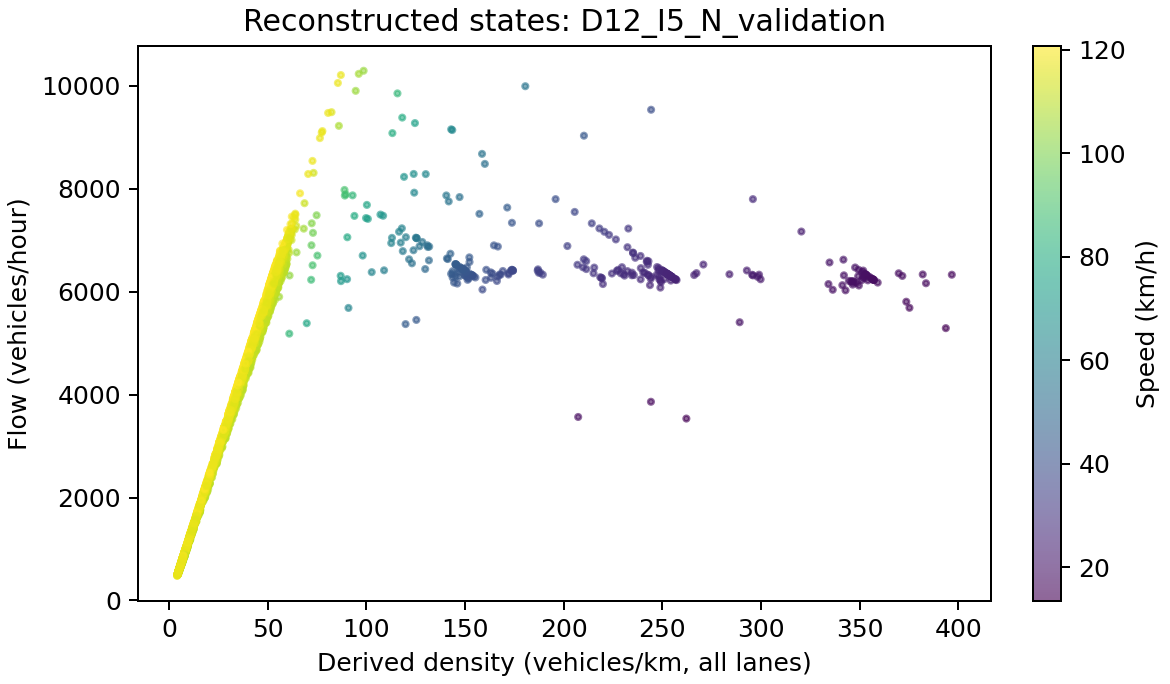
\includegraphics[width=\columnwidth]{fundamental_diagram.png}
\caption{Speed-colored reconstructed flow and derived density for the saved validation-state array. These are predictions, not hidden reference states.}\end{figure}
\begin{figure}[t]\centering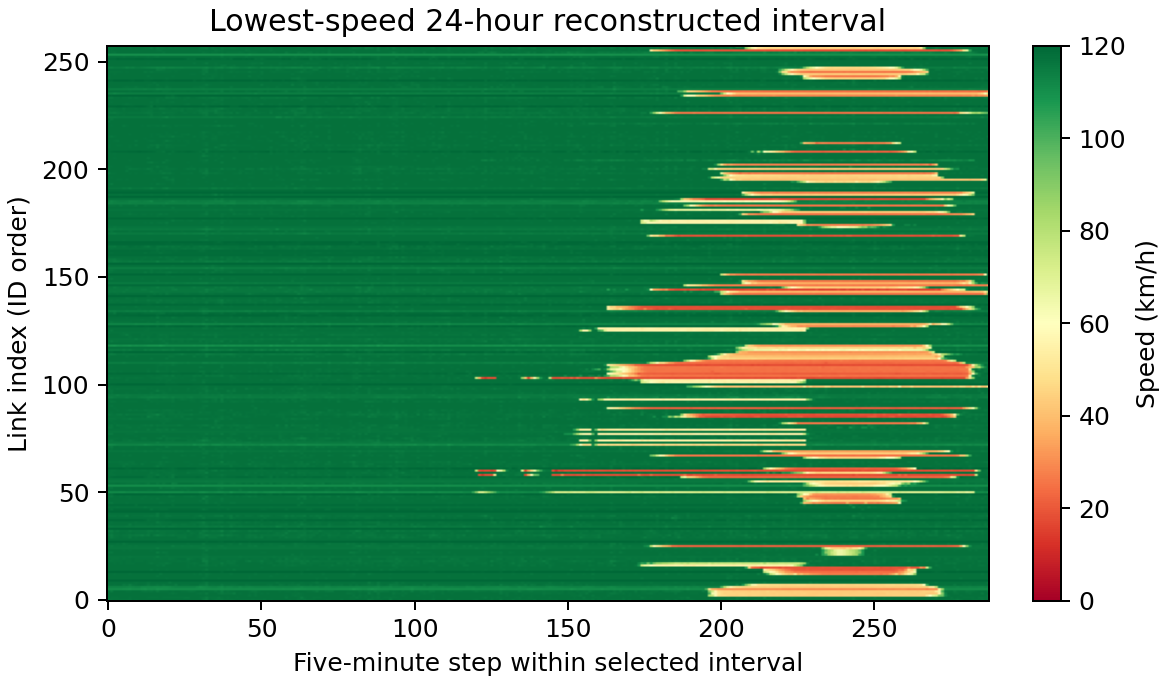
\includegraphics[width=\columnwidth]{space_time.png}
\caption{The lowest-average-speed reconstructed 24-hour interval. Links are displayed in identifier order; the interval-selection rule is fixed in the reporting code.}\end{figure}


\section{Fifth revision: ongoing queue localization and soft physical calibration}
\subsection{Location and persistence features}
The ongoing model adds normalized link-identifier index, static link attributes,
causal threshold-exceedance persistence over four history widths, and directed
three-hop context. These features follow the spatial-context principle used by
Traffic4cast 2022's second-place solution\footnote{\url{https://mlumiste.com/technical/gradient-boosting-neurips/}}.
This is an independently evaluated adaptation; neither that solution's score nor
its data is transferred to this benchmark. A 320-round LightGBM classifier uses
31 leaves, regularization, and inverse-sampling weights that preserve each
window's class balance. Fits end before October, decoder/blend selection uses
October, and promotion requires more than 0.005 IoU gain on both November and
January. These are previously examined development months, not independent tests.
Five ongoing heads pass. Onset alternatives fail the frozen gate and are rejected.
Production refits use all nine training months, with a maximum of 256 ongoing
proxy events per panel. The queue-only candidate changes 647 of 174,000 queue
cells while preserving every onset, state and path-flow value.

\subsection{State and fundamental-diagram trade-off}
A soft adjustment chooses a nearby free-flow or congested triangular-FD state
using speed/flow error scales from the official state metric. October selects
a blend from zero, 0.05, 0.1, 0.2 and 0.4. A state-plus-FD utility uses official
weights 0.35 and 0.05; LWR consequences are not inferred from this surrogate.
Promotion requires a gain above 0.0001 on both later blocks, with state-score
loss below 0.002. Only I405 South passes, at weight 0.2. The other pilot fails.

\begin{table}[t]\centering
\caption{Official public composite ablation. Private results and component scores are unavailable.}
\begin{tabular}{lc}\hline
Entry & Public score\\\hline
Fourth revision & 0.83176\\
Localized ongoing queues & 0.83200\\
Ongoing plus gated soft FD & 0.83207\\\hline
\end{tabular}\end{table}
The 0.00024 queue-only gain is equivalent to approximately 0.0008 in official
queue score, subject to leaderboard rounding. It is much smaller than the
observed-speed proxy gains. This limits the evidence for generalization from
proxy labels to the withheld latent queue labels. The extra state/physics change
adds 0.00007 composite and does not identify its task-level source. The selected
entry remains far from the public leader at 0.93089 in the 1 November snapshot;
no winning rank or award eligibility is claimed.


\section{Wave-aware reconstruction and queue-motion experiments}
We evaluated two additions to the fifth-revision components using matched
prefix fits, October selection, and previously inspected November and January
development blocks. Directed shortest-path road distances align upstream
free-flow context and downstream congested-wave context. This follows the
propagation distinction underlying adaptive smoothing~\cite{treiber2002}.
The queue challenger adds causal speed trends, distances to visible queued
links, and horizon interactions. Queue results below concern ongoing
observed-speed proxies, not official latent queue labels.

\begin{table}[t]
\centering\caption{V7 development changes against matched component controls.
State entries are changes in regime-macro $S_{state}$; queue entries are changes
in ongoing-window proxy IoU. They are different metrics.}
\label{tab:v7}
\begin{tabular}{llrr}
\hline
Task & Direction & November & January \\
\hline
State & I5 North & +0.00114 & +0.00180 \\
State & I10 East & +0.00037 & +0.00030 \\
State & I5 South & +0.00013 & +0.00015 \\
Queue & I5 North & +0.02000 & +0.00139 \\
Queue & I10 East & +0.00184 & +0.00330 \\
\hline
\end{tabular}
\end{table}

Only I5 North clears the registered state pilot minimum in both later blocks.
Its paired whole-day bootstrap, stratified by masking regime with fixed regime
weights, has positive fifth-percentile gains of 0.00080 and 0.00140.
All three regimes improve. These intervals condition on the selected candidate
and previously examined development data; they are not private-score confidence
intervals. I5 South does not replicate a gain large enough to pass the pilot.
Neither queue challenger clears the required 0.01 gain in both later blocks.
We retain the existing queue and OD components.

The I5 North state policy is refitted on all released training months.
Isolated submission 58021199 scores 0.83220, compared with the fifth-revision
reference at 0.83207. All queue, OD and other-panel state values are preserved,
so the 0.00013 composite change is attributable to the combined state and
physics contribution. The official breakdown is unavailable. Physics uses
hidden organizer boundary flows, so the local state gain alone cannot certify
its effect. This small public improvement does not establish a private gain.
At that stage, the fifth-revision entry was retained as a fallback.

\section{Attributed public-source extension}
\subsection{Sources and experimental boundary}
On 6 November we screened public repositories and model assets. The organizer
repository was already current at our pinned revision. The public
happyc0der reconstruction function was evaluated on the same masks and temporal
blocks as our prefix-fitted models, with its link axis restored to topological
order. In all twelve panel/block comparisons on I5 North, I5 South and I10 East,
our retained architecture scored higher; public-only macro $S_{state}$ was
0.0137--0.0316 lower. This compares algorithms under our common quality filter,
not the author's complete pipeline. The source has no detected reuse license,
so no part of it enters the delivery. The February audit week was untouched by
the v7 pilot but had appeared in earlier project work; it is not a pristine test.

The anubisyy assets declare CC0-1.0 in their primary Kaggle metadata and include
training code, model weights and a public inference notebook \cite{anubis}.
We regenerate its predictions locally rather than importing a submitted CSV.
Its historical 0.86517 is an author-reported reference; our regenerated file has
a different checksum and is not assigned that historical score. No complete
external entry is submitted as our own. Our hybrids retain our demand solver
and a substantive independent state component, with external attribution.

\subsection{Controlled component comparisons}
Let $(v_o,q_o)$ denote our retained state model and $(v_c,q_c)$ the public
CatBoost estimator. The predeclared midpoint candidate uses
\begin{equation}
(v,q)=0.5(v_o,q_o)+0.5(v_c,q_c).
\end{equation}
The public queue ensemble uses training-fitted LightGBM and CatBoost onset
checkpoints and a LightGBM ongoing checkpoint. Features use released history
strictly before the forecast origin. Neither offline state model feeds queues.
Independent replay matches all 174,000 queue predictions. Appending post-origin
rows preserves the extracted inputs exactly on all 160 windows; float32 feature
reductions differ by at most $2.39\times10^{-7}$ when memory layout changes.

\begin{table}[t]
\centering\caption{Measured public component comparisons. OD is our solver in every row.}
\begin{tabular}{lrr}
\hline
Candidate & Submission & Composite\\\hline
Our original v7 & 58021199 & 0.83220\\
Our states, public queues & 58063539 & 0.85777\\
Midpoint states, our queues & 58063563 & 0.83882\\
Midpoint states, public queues & 58063635 & 0.86438\\
Three-family states, public queues & 58067798 & 0.87387\\\hline
\end{tabular}
\end{table}
The queue-only gain is 0.02557 and the state/physics gain is 0.00662.
The combined improvement is 0.03218, consistent with additive scoring and
five-decimal rounding. These are controlled public submissions, not independent
private validation; public model selection can overfit that month. Full official
task breakdowns remain unavailable. The BizAI MIT release supplies a three-seed U-Net2 (width 48, 576-step context) \cite{bizai}. We infer its weights locally, streaming train-only weekday profiles and retaining the published link ordering. The final three-family state is $0.25(v_o,q_o)+0.25(v_c,q_c)+0.50(v_u,q_u)$; queue and OD remain unchanged. Submission 58067798 scores 0.87387, another 0.00949 public gain. This uses model weights rather than the author's saved component predictions. Its 0.88369 full-entry score belongs to that team and is not our reproduced result. A packaged replay authenticates the unchanged earlier full v7 checkpoint replay, regenerates the public components from weights, and compares all 6,980,503 values with the selected file. Queue and OD values match exactly; the maximum state difference is $5.46\times10^{-12}$ from floating-point serialization. The entry script also supports a fresh v7 replay rather than reusing the authenticated component. The credited external software, checkpoints,
versions, replay commands and licenses accompany the package.

\section{Conclusion}
The independent graph--temporal and wave-aware system establishes a fully
reproduced baseline. A licensed public queue component and a state ensemble
improve its measured public composite to 0.87387 after the U-Net addition, while retaining our OD solver.
The campaign preserves negative comparisons and separates model disagreement,
proxy validation and official public results. The private score and award
outcome remain unknown.

\section{Limitations and release statement}
Graph-masked attention with a temporal Transformer underperformed tree-only
reconstruction on the family-macro artificial-mask holdout (Table~II); the hybrid
blend also trailed unblended trees on nine-panel coverage. Neural training used
a single short epoch to fit memory limits, so the comparison favors trees on
compute as well as accuracy. The initial refinement selection accepted two panels; subsequent residual and enhanced-context policies promoted all ten after development-block review.
The implementation aggregates multiple stations on a link before learning,
which can lose station-specific variation even though final targets retain
station identifiers. Its dense graph attention can become expensive on large
panels. The reader processes one corridor at a time but holds that corridor's
selected date range in memory, so available RAM constrains full-training runs.
The synthetic benchmark does not establish generalization to measured traffic.
The strict merger checks the full official upload template and fails on missing values. There is no evidence yet about private leaderboard rank, and no claim that the selected hyperparameters are globally optimal. Queue proxies can disagree with latent labels, and the reported temporal proxy blocks participate in retention. No task-level official score can be recovered from these local comparisons.

Code uses the organizer's MIT-licensed evaluator utilities with attribution and the separately credited CC0 public model assets and MIT BizAI U-Net code/weights;
data remains governed by the competition rules. No hidden queue labels or private reference paths are requested or used.
AI assistance was used to implement this system and draft these notes. The author is responsible for the final verification and compliance with the competition publication rules.

\bibliographystyle{IEEEtran}
\bibliography{references}
\end{document}
